\chapter{Time Evolution}
Recall the expression for the superfluid state
\begin{equation}\label{eq:SF_psi}
\lvert \psi \rangle = C \sum_{j=0}^{\infty} \frac{\alpha^j}{\sqrt{j!}}\lvert j\rangle,
\end{equation}
Recent experimental advances have made it possible to change the Hamiltonian almost instantaneously, allowing for a wide array of new experiments. In the current section, we will look at the case of an SF Hamiltonian,
\begin{equation}\label{eq:SF_ham}
\hat{H} = -J \sum_{\braket{i,j}} \hat{a}_{i}^{\dag} \hat{a}_j,
\end{equation}
 present long enough for the condensate to reach the ground state in eq. \ref{eq:SF_psi} suddenly being switched to a pure Mott Hamiltonian,
\begin{equation}
 \hat{H} = \frac{U}{2} \sum_{i} \hat{n}_i \left( \hat{n}_i -1 \right).
\end{equation}
%
In this case, the time evolution of the state can be described by
\begin{equation}
\lvert \psi (t) \rangle = C \sum_{j=0}^{\infty} \e^{-it \frac{U}{2} j(j-1)}\frac{\alpha^j}{\sqrt{j!}}\lvert j\rangle,
\end{equation}
and since $j(j-1)/2\in \mathbb{N}$ for all $j$, we will regain the superfluid state at times $p2\pi/U$,
\begin{equation}
\lvert \psi (p2\pi/U) \rangle = \lvert \psi (0) \rangle,
\end{equation}
for all integers $p$, whereby we should see a revival of the condensate fraction, as described in \ref{CondFrac}.

\section{Numerical Results}
Further testing the applicability of the MPS formalism using ITensor library for time evolution, we evolved an SF state in time first with respect to a pure Mott Hamiltonian ($U=1$, $J=0$), then with respect to a slightly different Hamiltonian ($U=2$, $J=0.03$).

\subsection{$U=1$, $J=0$}
Mott time evolution on a superfluid state was performed for various unit occupancy systems with complex time steps $t_{1,2}=\frac{1\pm i}{2}t$ as described in \cite{cmplx_t}, and the condensate fraction was subsequently plotted as a function of time. The initial SF state was found by DMRG with the Hamiltonian in eq. \ref{eq:SF_ham}.
\begin{figure}[h!]
    \centering
    \begin{subfigure}[t]{0.49\textwidth}
        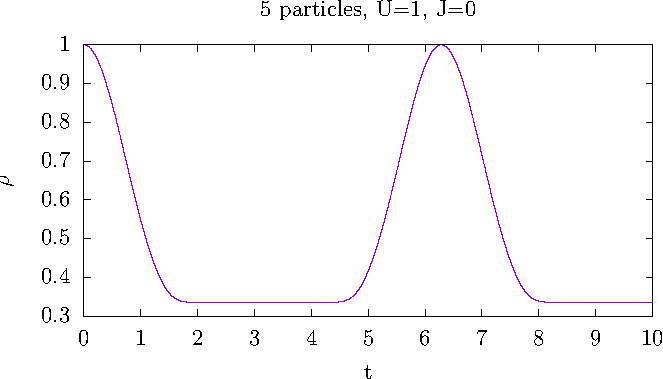
\includegraphics[width=\textwidth]{Figures/TimeEvo5_U1_J0.pdf}
        \caption{\textit{Condensate fraction calculated from a 5 particle, 5 site MPS after performing 10 DMRG sweeps with an SF Hamiltonian ($J=1$, $U=0$) followed by time evolution with a Mott Hamiltonian ($J=0, U=1$).}}
        \label{fig:TimeEvo5_U1_J0}
    \end{subfigure}
    ~
    \begin{subfigure}[t]{0.49\textwidth}
        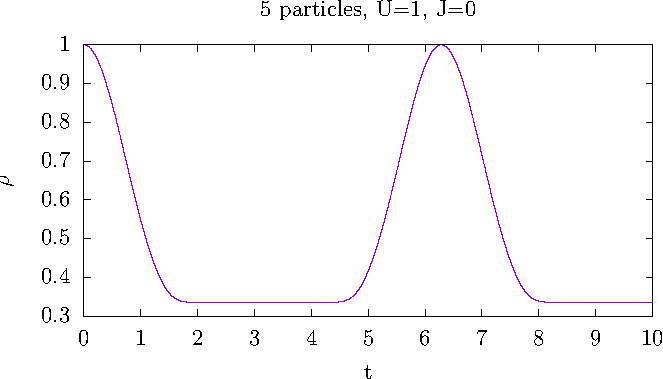
\includegraphics[width=\textwidth]{Figures/TimeEvo50_U1_J0.pdf}
        \caption{\textit{Condensate fraction calculated from a 50 particle, 50 site MPS after performing 20 DMRG sweeps with an SF Hamiltonian ($J=1$, $U=0$) followed by time evolution with a Mott Hamiltonian ($J=0, U=1$).}}
        \label{fig:TimeEvo50_U1_J0}
    \end{subfigure}    
\end{figure}
Figure \ref{fig:TimeEvo5_U1_J0} shows time evolution for 5 particles, whereas \ref{fig:TimeEvo50_U1_J0} is for 50 particles (note: figure not yet made). 

WAITING FOR DATA...

\subsection{$U=2$, $J=0.03$}
Performing time evolution on an SF state with a nonzero $J$, the condensate fraction does not achieve full revival, but instead the phases of the individual particle states interfere with each other more and more for each cycle, leading to a decreasing maximal condensate fraction and some spurious lumps in between the peaks, see fig. \ref{fig:TimeEvo5_U2_J0_03}. In fig. \ref{fig:ExDiagComp_U2_J0_03}, the absolute difference between the condensate fraction calculated by MPS formalism and that calculated by exact diagonalization is plotted. The disagreement, while still small at $t=10$, is expected to grow larger for larger times, as the MPS does a series of truncations each time the time evolution MPO is applied to avoid increasing the bond dimension of the MPS, whereas exact diagonalization using the Lanczos algorithm [Lanczos, C. "An iteration method for the solution of the eigenvalue problem of linear differential and integral operators", J. Res. Nat’l Bur. Std. 45, 255-282 (1950)] is limited mainly by machine precision.

\begin{figure}[h!]
    \centering
    \begin{subfigure}[t]{0.49\textwidth}
        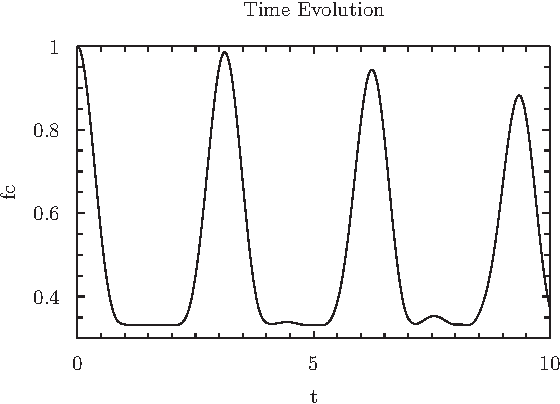
\includegraphics[width=\textwidth]{Figures/TimeEvo5_U2_J0_03.pdf}
        \caption{\textit{Condensate fraction calculated from a 5 particle, 5 site MPS after performing 10 DMRG sweeps with an SF Hamiltonian ($J=1$, $U=0$) followed by time evolution with a ($J=00.3, U=2$) Hamiltonian.}}
        \label{fig:TimeEvo5_U2_J0_03}
    \end{subfigure}
    ~
    \begin{subfigure}[t]{0.49\textwidth}
        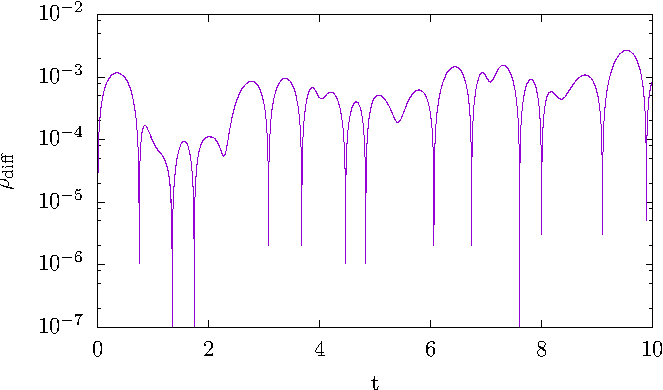
\includegraphics[width=\textwidth]{Figures/TimeEvo5_U2_J0_03_VS_ExactDiag.pdf}
        \caption{\textit{Condensate fraction calculated from a 5 particle, 5 site MPS after performing 10 DMRG sweeps with an SF Hamiltonian ($J=1$, $U=0$) followed by time evolution with a ($J=0.03, U=2$) Hamiltonian compared with the same calculations done with exact diagonalization.}}
        \label{fig:ExDiagComp_U2_J0_03}
    \end{subfigure}
\end{figure}

%Consider the Bose-Hubbard Hamiltonian
%\begin{equation}
%	\hat{H} = -J \sum_{\braket{i,j}} \hat{a}_{i}^{\dag} \hat{a}_j + \frac{U}{2} \sum_{i} \hat{n}_i \left( \hat{n}_i -1 \right) \; , 
%\end{equation}
%which describes nearest-neighbour interactions in a one-dimensional lattice. This Hamiltonian supports two distinct quantum phases: The Superfluid (SF) phase, $U/J \ll 1$, which exhibit long range correlations, and the Mott-Insulator (MI) phase, $U/J \gg 1$, where sites are isolated, hence no correlation between sites is present. The SF phase is a Bose-Einstein condensate with special attributes, as it exhibits maximal de-localization of the particles and can be approximated as a coherent state. On the other hand, as the individual sites are completely decoupled in the MI phase, no condensate is present. \\
%According to the Penrose-Onsager criterion, a Bose-Einstein condensate, and by extension the SF state, is present if and only if the largest eigenvalue, $\lambda_1$, of the single-particle density matrix, $\rho^{(1)}$, is macroscopic
%\begin{equation}
%	f_c = \frac{\lambda_1}{N_{\mathrm{particles}}} > 0 \; ,
%\end{equation} 
%where $f_c$ is the \textit{condensate fraction} and $N_{\mathrm{particles}}$ is the total number of particles. Thus, the condensate fraction can be used to determine which state is the dominant of the system, as
%\begin{align}
%	\lim_{N_{\mathrm{particles}} \to \infty} f_{c}^{\mathrm{SF}} &\to 1 \label{eq:SF_lim} \\
%	\lim_{N_{\mathrm{particles}} \to \infty} f_{c}^{\mathrm{MI}} &\to 0 \; , \label{eq:MI_lim}
%\end{align}
%where the filling-fraction $n = N_{\mathrm{particles}}/N_{\mathrm{sites}}$ is held constant. While the limit for the SF phase will be reached for any number of particles, the MI phase will only be reached in the limit $N_{\mathrm{particles}} \to \infty$.
%
%\section{Numerical Results}
%In order to test the precision of MPS formalism and the ITensor library, the condensate fraction was calculated for a series of $U/J$ with varying particle number. For this the library's DMRG algorithm was used, where the number of sweeps was selected such that the bond dimension remained the same when adding more sweeps. In this case 5 sweeps with a maximum bond dimension of 200 was sufficient. All calculations were performed with unit occupancy. These results were then compared to a similar calculation using exact diagonalisation.
%
%\begin{figure}[h!]
%    \centering
%    \begin{subfigure}[t]{0.49\textwidth}
%        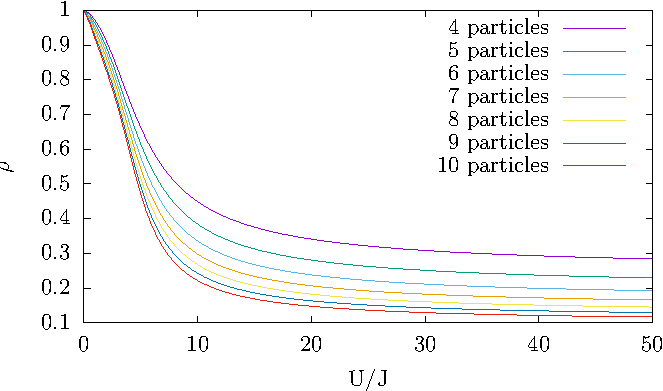
\includegraphics[width=\textwidth]{Figures/Condfrac_4to10.pdf}
%        \caption{\textit{Condensate fraction calculated from an MPS after performing 5 DMRG sweeps.}}
%        \label{fig:Condfrac_4to10}
%    \end{subfigure}
%    ~
%    \begin{subfigure}[t]{0.49\textwidth}
%        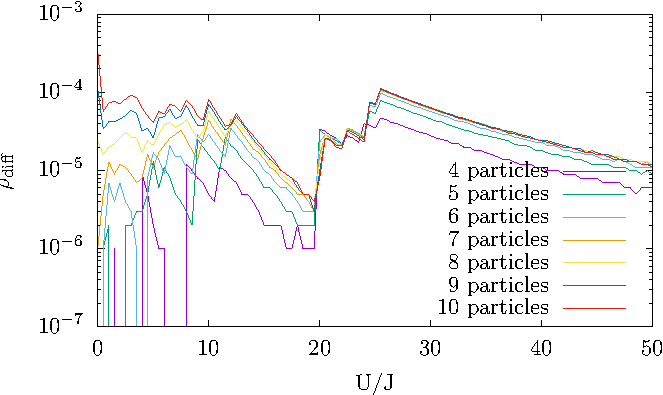
\includegraphics[width=\textwidth]{Figures/Confrac_exactvsMPS.pdf}
%        \caption{\textit{Absolute difference between the condensate fraction calculated using MPS and using exact diagonalisation.}}
%        \label{fig:Condfrac_exactvsMPS}
%    \end{subfigure}    
%\end{figure}
%Figure \ref{fig:Condfrac_4to10} shows the condensate fraction for various $U/J$ calculated using MPS. In the limit $U/J = 0$ the condensate fraction is 1 as expected, thus confirming that the system is in the SF state. Meanwhile, in the limit $U/J = 50$ the condensate fraction is dependent on the number of particles, however, this is just as equation \ref{eq:MI_lim} describes.\\
%In figure \ref{fig:Condfrac_exactvsMPS} the results of the MPS calculation is compared to exact diagonalisation by displaying the absolute difference between the two calculations. It is clear that the two approaches yield very similar results for low particle-number.\\
%One of the great advantages of MPS is its ability to accurately describe states with a large number of particles, which is unfeasible with exact diagonalisation. 
%\begin{figure}[h!]
%	\centering
%	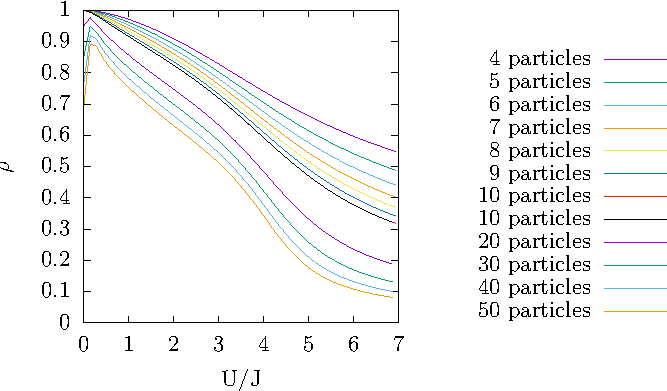
\includegraphics[width=0.9\textwidth]{Figures/Condfrac_4to50.pdf}
%	\caption{\textit{Condensate fraction calculated from an MPS after performing 5 DMRG sweeps.}}
%	\label{fig:Condfrac_4to50}
%\end{figure}
%Figure \ref{fig:Condfrac_4to50} shows the results of the DMRG calculations for up to 50 particles. The condensate fraction behaves as expected in the $U/J \gg 1$ limit, as it tends towards zero for larger particle numbers. Note, however, that in the SF limit the results are not at all as described by equation \ref{eq:SF_lim}. This is due to a flaw of the MPS approximation, as correlation functions of an MPS approximation \textit{always} decay exponentially with respect to distance, thus limiting the correlation length $\xi$. As the system grows in size, its length exceeds the correlation length of the approximated MPS, which becomes an issue when describing a pure SF state, as it exhibits very long range correlations. Thus, the MPS is unable to describe the long-range correlation functions of the SF state, resulting in the abnormal behaviour of the result in the $U/J \ll 1$ limit.
%
%\subsection{Visualization of density matrices}
%One way of displaying the correlations of the system is to plot its density matrix, whose entries are given by
%\begin{equation}
%	\rho_{i,j} = \bra{\psi} \hat{a}_{i}^{\dag} \hat{a}_j \ket{\psi} \; .
%\end{equation}
%\begin{figure}[h!]
%    \centering
%    \begin{subfigure}[t]{0.49\textwidth}
%        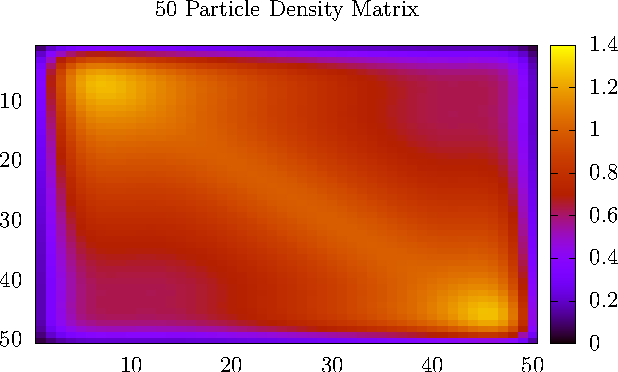
\includegraphics[width=\textwidth]{Figures/DensityMatSF.pdf}
%        \caption{\textit{Norm value of density matrix entries for $U/J = 0.1$.}}
%        \label{fig:DensityMatSF}
%    \end{subfigure}
%    ~
%    \begin{subfigure}[t]{0.49\textwidth}
%        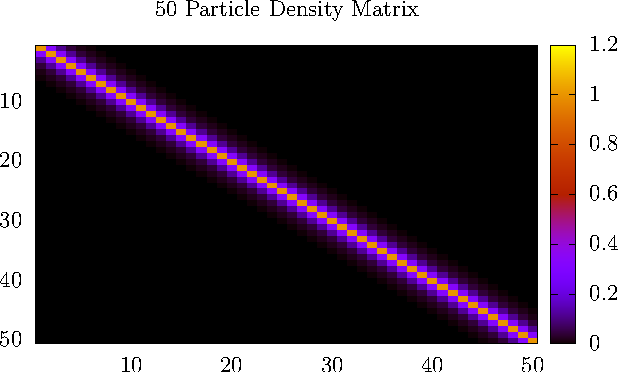
\includegraphics[width=\textwidth]{Figures/DensityMatMI.pdf}
%        \caption{\textit{Norm value of density matrix entries for $U/J = 12$.}}
%        \label{fig:DensityMatMI}
%    \end{subfigure}    
%\end{figure}
%Figures \ref{fig:DensityMatSF} and \ref{fig:DensityMatMI} show the density matrix of the 50 particle system plotted for the Superfluid and the Mott-Insulator limit respectively. In the SF limit long-range correlations are present, which is seen by large off-diagonal elements. However, as discussed previously, in the MPS approximation all correlations decay exponentially, which causes issues for the elements furthest from the diagonal (top-right and bottom-left corner). In the MI limit no interaction takes place between sites and the correlation length is zero,  leading to a correlation matrix consisting only of diagonal elements of equal magnitude. Figure \ref{eq:MI_lim} shows some off-diagonal elements of low, but not zero, magnitude, since it is made for $U/J = 12$, meaning the system is not a pure Mott-Insulator.